\section{Auswertung}
Da es Ziel des Versuches ist, den Diffusionskoeffizienten $D$ zu berechnenen müssen zunächst die beiden 
Relaxationszeiten $T_1$ und $T_2$ bestimmt werden. In einem letzten, vergleichenden Schritt wird dann 
der Molekülradius von Wasser bestimmt.
Zu Beginn beträgt die Temperatur an der Probenposition $T = 22,4\,\symup{°C}$. 
\subsection{Bestimmung der Spin-Gitter Relaxationszeit} 
Zur Berechnung der Relaxationszeit $T_1$ wird zunächst ein 180°-Puls durchgeführt, woraufhin ein 90°-Puls 
nach der Zeitspanne $\tau$ folgt. Die dadurch gemessenen Spannungen sind für verschiende $\tau$ in \autoref{tab:t1} im Anhang
zu sehen. \\
Nach \autoref{eq:T1} wird eine Ausgleichskurve der Form 
\begin{equation*}
    M(\tau) = M_0 \cdot \exp \left( -\frac{\tau}{T_1} \right) + M_1
\end{equation*}
bestimmt. Hierzu und auch für folgende Rechnungen wird die Python 3.8 Bibliothek \textit{SciPy}\cite{scipy}
verwendet. Die Datenpunkte, sowie die Ausgleichskurve sind in \autoref{fig:T1} grafisch dargestellt.
Die Ausgleichsparameter ergeben sich zu 
\begin{align*}
    M_0 &= (-1,83 \pm 0,05) \, \symup{V} \\
    M_1 &= (0,89 \pm 0,05) \, \symup{V} \\
    T_1 &= (2,41 \pm 0,18) \, \symup{s}.
\end{align*}
\begin{figure}
    \centering
    \includegraphics[width=0.6\textwidth]{build/plot_T1.pdf}
    \caption{Gemessene Spannungen aufgetragen gegen den Abstand der Impulse mit Ausgleichskurve zur Bestimmung von $T_1$.}
    \label{fig:T1}
\end{figure}

\subsection{Bestimmung der Spin-Spin Relaxationszeit}
Zu Beginn dieser Messung wurde eine Temperatur von $T = 21,7 \, \symup{°C}$ an der Probenposition gemessen.
Zur Bestimmung der Spin-Spin Relaxationszeit $T_2$ wird hier die Meiboom-Gill Methode verwendet.
Der gemessene Amplitudenverlauf in Abhängigkeit der Zeit ist in \autoref{fig:T2} dargestellt.
Mittels der Python 3.8 Bibliothek \textit{SciPy}\cite{scipy} werden die Maxima des Verlaufs gefunden.
Durch diese wird nach \autoref{eq:T2} eine Ausgleichskurve der Form 
\begin{equation*}
    M(t) = M_0 \cdot \exp \left(-\frac{t}{T_2} \right) + M_1
\end{equation*}
gelegt. Diese ist ebenfalls in \autoref{fig:T2} zu sehen.
Die Ausgleichsparameter ergeben sich zu 
\begin{align*}
    M_0 &= (0,65 \pm 0,01) \, \symup{V}\\
    M_1 &= (0,06 \pm 0,02) \, \symup{V}\\
    T_2 &= (1,03 \pm 0,07) \, \symup{s}.
\end{align*}
\begin{figure}
    \centering
    \includegraphics[width=0.6\textwidth]{build/plot_T2.pdf}
    \caption{Darstellung der gemessenen Spannungen mit eingezeichneten Maxima und Ausgleichskurve zur Bestimmung von $T_2$.}
    \label{fig:T2}
\end{figure}
Um genauere Ergebnisse zu erhalten, wäre eine exakte Einstellung der Pulslänge für den 180°-Puls notwendig.
Diese Carr-Purcell Methode ist in der Praxis allerdings nicht umsetzbar und würde zu großen Fehlern führen.
Eine so getätigte Messung ist in \autoref{fig:mgoff}
zu sehen. Mit diesen Daten lässt sich $T_2$ nicht bestimmen.
\begin{figure}
    \centering
    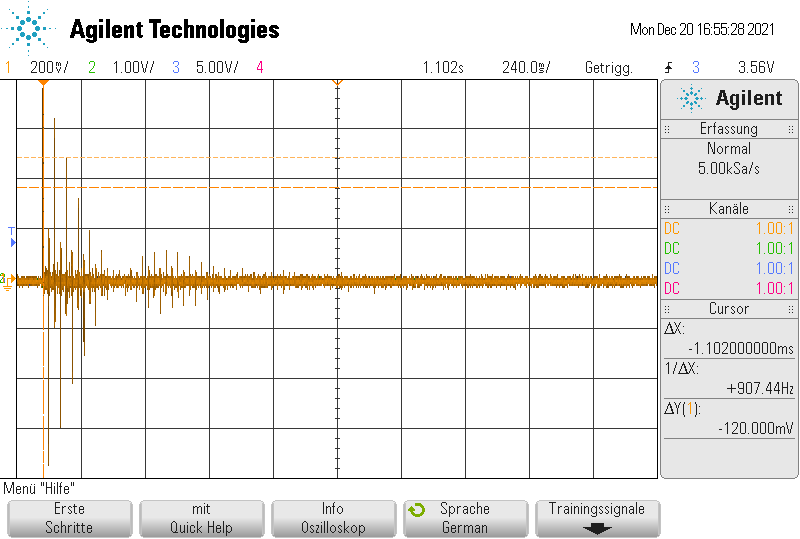
\includegraphics[width=0.6\textwidth]{data/ohnemg.png}
    \caption{Darstellung der gemessenen Spannungen mit der Carr-Purcell-Methode.}
    \label{fig:mgoff}
\end{figure}

\subsection{Bestimmung des Diffusionskoeffizienten}
Zur Bestimmung des Diffusionskoeffizienten $D$ über \autoref{eq:D} werden sowohl die Gradientenstärke $G$
als auch die Zeitkonstante $T_D$ benötigt. Beide Größen lassen sich im Folgenden bestimmen.
Vor dieser Messung lag die Temperatur bei $T = 21,4 \, \symup{°C}$\\

Zunächst wird die Gradientenstärke $G$ berechnet. Dazu wird der Gradient entlang der z-Achse maximiert und 
ein gut sichtbares Echo bei $\tau = 0,005\, \symup{s}$ aufgenommen. Dieses Echo ist in \autoref{fig:echo}
zu sehen.
\begin{figure}
    \centering
    \includegraphics[width=0.6\textwidth]{build/Echo.pdf}
    \caption{Darstellung des gemessenen Echos bei $\tau = 0,005\,\symup{s}$ zur Bestimmung von $D$.}
    \label{fig:echo}
\end{figure}
Zur Bestimmung des Diffusionskoeffizienten muss eine Fouriertransformation durchgeführt werden, wobei 
alle Werte vor dem Maximum des Realteils verworfen werden. Die Fouriertransformation ist stark vergrößert 
in \autoref{fig:fft} zu sehen.
\begin{figure}
    \centering
    \includegraphics[width=0.6\textwidth]{build/echo_gradient.pdf}
    \caption{Darstellung der Fouriertransformation des gemessenen Echos bei $\tau = 0,005\,\symup{s}$.}
    \label{fig:fft}
\end{figure}
Der Durchmesser des Halbkreises ist dabei ungefähr
\begin{equation*}
    d_f \approx 14174,72 \,\frac{1}{\symup{s}}.
\end{equation*}
Damit ergibt die Gradientenstärke zu 
\begin{equation*}
    G = \frac{2 \pi \cdot d_f}{\gamma \cdot d} = 0,079 \, \frac{\symup{T}}{\symup{m}},
\end{equation*}
wobei $\gamma = 2,675 \cdot 10^{8} \, \frac{1}{\symup{s T}}$ das gyromagnetische Verhältnis von Protonen\cite{gamma} und 
$d = 0,0042\,\symup{m}$ der Probendurchmesser ist.\\

Die Zeitkonstante $T_D$ lässt sich über die Messwerte aus \autoref{tab:diff} berechnen.
Zunächst wird dabei eine rein quantitave Überprüfung der Messwerte vorgenommen.
Dazu wird eine lineare Regression der Form 
\begin{equation*}
     \text{ln}(M(\tau)) - 2\tau /T_2 = a \tau^3 + b
\end{equation*}     
durchgeführt,
was in \autoref{fig:quanti} zu sehen ist.
Wie zu sehen ist, folgen die gemessenen Werte der Gerade sehr grob, wobei der erste Wert aus \autoref{tab:diff}
hierbei rausgenommen wurde und auch im folgenden Auswertungsteil weggelassen wird, da die Abweichung zur Gerade 
sehr groß war.
Die Parameter ergeben sich zu 
\begin{align*}
    a = (-0,0046 \pm 0,0004) \, \symup{ms}^3 \\
    b = -11,6 \pm 1,4.
\end{align*}
Damit ließ sich die $\tau**3$-Abhängigkeit zumindest grob bestätigen.\\
\begin{figure}
    \centering
    \includegraphics[width=0.6\textwidth]{build/quanti.pdf}
    \caption{Darstellung einer quantitativen Überprüfung der Messwerte mit eingzeichneter Ausgleichsgerade.}
    \label{fig:quanti}
\end{figure}
Zur Bestimmung der Zeitkonstante $T_D$ wird nun eine Ausgleichskurve der Form 
\begin{equation*}
    M(\tau) = M_0 \cdot \exp \left( - \frac{2 \tau}{T_2}  \right) \exp \left( - \tau^3 \cdot H   \right) + M_1
\end{equation*}
durchgeführt, wobei $H$ eine eingeführte Hilfsgröße mit 
\begin{equation*}
    T_D = \frac{1}{\tau^2 H}
\end{equation*}
ist. Dies ist in \autoref{fig:TD} zu sehen.
Die Ausgleichsparameter lauten
\begin{align*}
    M_0 &= (0,649 \pm 0,005) \, \symup{V} \\
    M_1 &= (0,053 \pm 0,005) \, \symup{V} \\
    H   &= (649846 \pm 15884) \, \frac{1}{\symup{s^3}}.
\end{align*}
Mit \autoref{eq:D} ergibt sich dadurch der Diffusionskoeffizient zu
\begin{equation*}
    D = \frac{3 H}{2 \gamma^2 G^2} = (2,18 \pm 0,05 ) \cdot 10^{-9} \, \frac{\symup{m^2}}{\symup{s}}.
\end{equation*}
\begin{figure}
    \centering
    \includegraphics[width=0.6\textwidth]{build/plot_TD.pdf}
    \caption{Darstellung der Messwerte zur Bestimmung des Diffusionskoeffizienten mit Ausgleichskurve.}
    \label{fig:TD}
\end{figure}

\subsection{Berechnung des Molekülradius}
Der Molekülradius von Wasser wird mittels der Einstein-Stokes-Formel \autoref{eq:R0} berechnet. 
Die verwendete Viskosität des Wassers ist $\eta = 1002 \cdot 10^{-6}\, \frac{\symup{kg}}{\symup{m s}}$ \cite{visko}
bei 20\,°C. Zum Zeitpunkt des Versuchs wurde eine Temperatur von $21,4\, °\symup{C}$ gemessen.
Trotz der Temperaturdiskrepanz zwischen gemessener Temperatur und zur Viskosität gehörender Viskosität 
wird hier mit diesem Wert gearbeitet. Der Molekülradius ergibt sich somit zu 
\begin{equation*}
    r_{\text{gem}} = (0,98 \pm 0,02) \, \symup{\mathring{A}}. 
\end{equation*} 
Eine andere Möglichkeit, den Molekülradius zu berechnen ergibt sich über die Dichte $\rho = 998,21 \,\frac{\symup{kg}}{\symup{m}^3}$
und der Molekulardichte $M_W = 0,0180152 \, \frac{\symup{kg}}{\symup{mol}}$ von Wasser\cite{visko}.
Dabei wird angenommen, dass hexagonal dichteste Kugelpackungen vorliegen, also eine Raumfüllung von $74\%$.
\begin{equation*}
    r_{\text{hdk}} = \sqrt[3]{\left( \frac{M_W}{4/3 \pi \rho N_A}  \right)} = 1,74 \, \symup{\mathring{A}},
\end{equation*}
wobei $N_A$ die Avogadro-Konstante ist.